\documentclass[12pt]{exam}

\newcommand{\course}{MTH 234 Summer 2021}
\newcommand{\qdate}{15.1 - Double Integrals over Rectangles} %PUT DATE HERE
\newcommand{\quiz}{Group Work} 

    \usepackage[top=1in, bottom=1in, left=.45in, right=.45in]{geometry}
    \usepackage{amsmath,amsthm,amssymb,amstext}
    \usepackage{enumerate,enumitem}
    \usepackage{tikz,float,graphicx}
    \usepackage{microtype}
    \usepackage{bm,tikz}
        \usetikzlibrary{calc,positioning}
    \usepackage{multicol}
    \usepackage{nicematrix}
    \usepackage{cleveref}
    \usepackage[framemethod=tikz]{mdframed}
    \usepackage{graphicx}
    \usepackage[export]{adjustbox}
    
    %\newcommand{\course}{MTH 234 Summer 2021}
    %\newcommand{\qdate}{Equations of lines and planes} %PUT DATE HERE
    %\newcommand{\quiz}{Group Work} 
    
    \newcommand{\R}{\mathbb{R}}
    
    \newcommand{\ba}{\bm{a}}
    \newcommand{\bb}{\bm{b}}
    \newcommand{\bc}{\bm{c}}
    \newcommand{\bi}{\bm{i}}
    \newcommand{\bj}{\bm{j}}
    \newcommand{\bk}{\bm{k}}
    \newcommand{\br}{\bm{r}}
    \newcommand{\bv}{\bm{v}}
    \newcommand{\bu}{\bm{u}}
    \newcommand{\gen}[1]{\left\langle #1 \right\rangle}
    \newcommand{\pd}[2]{\dfrac{\partial #1}{\partial #2}}

\newtheorem*{theorem}{Theorem}
\surroundwithmdframed[]{theorem}

\theoremstyle{definition}
    \newtheorem*{definition}{Definition}
    \surroundwithmdframed[]{definition}
    \newtheorem*{info}{Useful Information}
    \surroundwithmdframed[]{info}
\theoremstyle{remark}
    \newtheorem*{remark}{Remark}
    \surroundwithmdframed[]{remark}
    

%%%%%%%%%%%%%%%%%%%%%%%
% HEADER AND FOOTER
%%%%%%%%%%%%%%%%%%%%%%%
\pagestyle{headandfoot}
\firstpageheadrule
\runningheadrule
\firstpageheader{\course}{\quiz}{\qdate}
\runningheader{\course}{\quiz}{\qdate}
\runningfooter{}{}{}


\usepackage{color}
\shadedsolutions
\definecolor{SolutionColor}{rgb}{0.8,0.9,1}

\usepackage{pgfplots}
    \pgfplotsset{every axis/.append style={
                    axis x line=middle,    % put the x axis in the middle
                    axis y line=middle,    % put the y axis in the middle
                    axis z line=middle,
                    axis line style={<->}, % arrows on the axis
                    xlabel={$x$},          % default put x on x-axis
                    ylabel={$y$},          % default put y on y-axis
                    zlabel={$z$},
                    grid=both,
                    %xtick={-4,...,-1,1,...,3},
                    %ytick={-1,1,}
    }}
    \pgfplotsset{compat=1.17}

\newcommand{\bif}{\quad\iff\quad}

%\printanswers
\noprintanswers

\begin{document}

\section*{\qdate}

%\subsection*{Template}

\begin{questions}

\question Extimate the volume of the solid that lies below the surface 
\(z=xy\) and above the rectangle contained in the \(xy\)-plane \(R=[0,6]\times[0,4]\). Use \(\Delta x=3\) and \(\Delta y=2\) and each sample point \((x_k,y_k)\) is the upper right corner of the $k$th rectangle.

\begin{minipage}[b]{.4\textwidth}

\emph{\(R\) is drawn to the right with dashed lines representing the appropriate rectangles and the sample points are marked.}

\ifprintanswers
    \begin{solution}
    \end{solution}
\else
    \vspace{7.5cm}
    \fi

\end{minipage}~
\begin{minipage}[t]{.5\textwidth}
    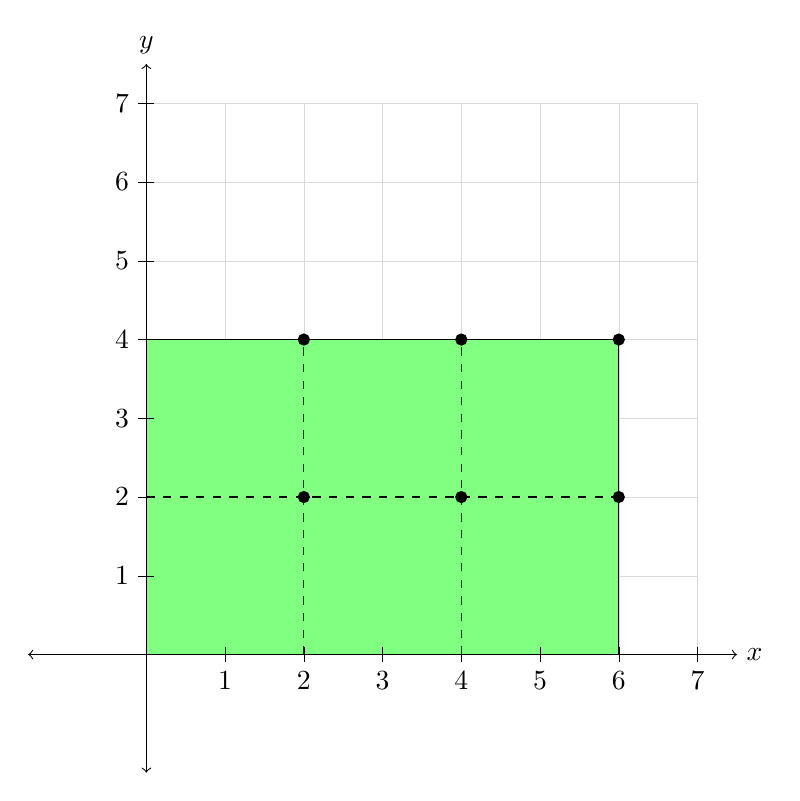
\begin{tikzpicture}
        \draw[very thin,gray!30] (0,0) grid (7,7);
        \draw[thin,<->] (-1.5,0)--(7.5,0) node[right] {$x$};
        \draw[thin,<->] (0,-1.5)--(0,7.5) node[above] {$y$};
        \draw[fill=green!50] (0,0)--(6,0)--(6,4)--(0,4)--(0,0);

        \foreach \x in {1,2,3,4,5,6,7}{
            \draw[very thin] ($ (\x,0) + (0,1mm) $) -- ($ (\x,0) - (0,1mm) $) node[below] {$\x$};
        }

        \foreach \y in {1,2,3,4,5,6,7}{
            \draw[very thin] ($ (0,\y) + (1mm,0) $) -- ($ (0,\y) - (1mm,0) $) node[left] {$\y$};
        }
        \foreach \x in {2,4}{
            \draw[dashed] (\x,0)--(\x,4);
        }
        \draw[dashed] (0,2)--(6,2);

        \foreach \x/\y in {2/2,2/4,4/2,4/4,6/2,6/4}{
            \draw[fill=black] (\x,\y) circle[radius=2pt];
        }
    \end{tikzpicture}
\end{minipage}

\question Estimate \(\int\int_{R}\sin(x+y)~ dA\) where \(R=[0,\pi]\times[0,\pi]\) taking sample points at the lower left corners of each rectangle.
\ifprintanswers
        \begin{solution}
        \end{solution}
    \else
        \vfill
    \fi

\newpage

\question Evaluate each double integral by identifying it as the volume of a solid and using a known formula
\begin{parts}
    \part \(\int\int_{R}3~dA\) where \(R=\{(x,y)~|~-2\le x\le 2, 1\le y \le 6\}\)
    \ifprintanswers
        \begin{solution}
        \end{solution}
    \else
        \vfill
    \fi 

    \part \(\int\int_{R}(4-2y)~dA\), \(R=[0,1]\times[0,1]\)

    \emph{Hint: First draw \(z=4-2y\) in the \(yz\)-plane and then use that to visualize what the portion of the plane \(z=4-2y\) looks like over the given region.}
    \ifprintanswers
        \begin{solution}
        \end{solution}
    \else
        \vfill
    \fi
\end{parts}

\end{questions}

\end{document}

% soln : Question environment
    \ifprintanswers
        \begin{solution}
        \end{solution}
    \else
        \vfill
    \fi